%  !TeX  root  =  user_guide.tex 

\section{Coordinate Capture Plugin}

% when the revision of a section has been finalized, 
% comment out the following line:
% \updatedisclaimer

The coordinate capture plugin is easy to use and provides the 
ability to display coordinates on the map canvas for two 
selected Coordinate Reference Systems (CRS).

\begin{figure}[ht]
   \begin{center}
   \caption{Coordinate Cature Plugin \nixcaption}\label{fig:coordinate_capture_dialog}\smallskip
   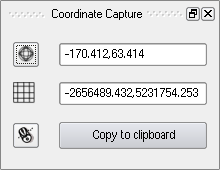
\includegraphics[clip=true, width=9cm]{coordinate_capture_dialog}
\end{center}  
\end{figure}

\begin{enumerate}
  \item Start QGIS, select \dropmenuopttwo{mActionOptions}{Project Properties} from 
  the \mainmenuopt{Settings} (KDE, Windows) or \mainmenuopt{File} (Gnome, OSX) menu 
  and click on the \tab{Projection} tab. As an alternative you 
  you can also click on the \toolbtntwo{mIconProjectionEnabled}{projector} icon in the lower 
  right-hand corner of the statusbar.
  \item Click on the \checkbox{Enable on the fly projection} checkbox and select a projected 
  coordinate system of your choice (see also Section \ref{label_projections}).
  \item Load the coordinate capture plugin in the Plugin Manager (see Section 
  \ref{sec:load_core_plugin}) and ensure that the dialog is visible by going to \mainmenuopt{View}
   > \dropmenuopt{Panels} and ensuring that \checkbox{Coordinate Capture} is enabled. 
   The cordinate capture dialog appears as shown in Figure \ref{fig:coordinate_capture_dialog}.
  \item Click on the \toolbtntwo{geographic}{Click to the select the CRS to use for coordinate display} 
  icon and select a different CRS from the one you selected above.
  \item To start capturing coordinates, click on \button{Start capture}. You can now click anywhere 
  on the map canvas and the plugin will show the coordinates for both of your selected CRS.
  \item To enable mouse coordinate tracking click the \toolbtntwo{tracking}{mouse tracking} icon.
  \item You can also copy selected coordinates to the clipboard.
\end{enumerate}

\newpage
